% !TEX root = ../main.tex
\section{Findings in Specific Subgroups}

	\subsection{Gender}

		\begin{table}[H]
      \centering
      \begin{tabular}{l || l | l || l | l || l | l }
        \hline
         & \multicolumn{2}{c||}{\bf Shopping} & \multicolumn{2}{c||}{\bf Smartphone} &\multicolumn{2}{c}{\bf Bank} \\ \hline
        {\bf Parameters}   & {\bf Male} & {\bf Female} & {\bf Male} & {\bf Female} & {\bf Male} & {\bf Female}\\ \hline
        \#Patterns         & 529    & 278    & 529    & 278    & 529    & 278  	 \\
        Avg. Size          & 5.684  & 5.263  & 5.465  & 5.270  & 6.089  & 5.572  \\
        Avg. Length        & 5.225  & 4.687  & 5.034  & 4.720  & 5.927  & 5.154  \\
        \#Intersections    & 147 		& 20     & 120    & 23     & 284    & 69     \\
        Avg. Intersections & 0.278  & 0.072  & 0.227  & 0.082  & 0.537  & 0.248  \\
        \#Overlaps         & 13     & 1      & 12     & 0      & 16     & 3  		 \\
        Avg. Overlaps      & 0.025  & 0.04   & 0.023  & 0      & 0.030  & 0.011  \\ \hline
        Avg. Strength      & 14.127 & 12.062 & 13.221 & 12.122 & 16.398 & 13.744 \\ 
        Min strength       & 6.339  & 6.339  & 6.339  & 6.339  & 6.339  & 6.339  \\
        Max strength       & 44.442 & 32.95  & 44.442 & 32.078 & 44.442 & 40.072 \\ \hline
      \end{tabular}
      \caption{Password strength and gender }
      \label{tab:gendertrength}
    \end{table}

    \begin{figure}[H]
    	\centering
    	\subfigure[Male]{
    		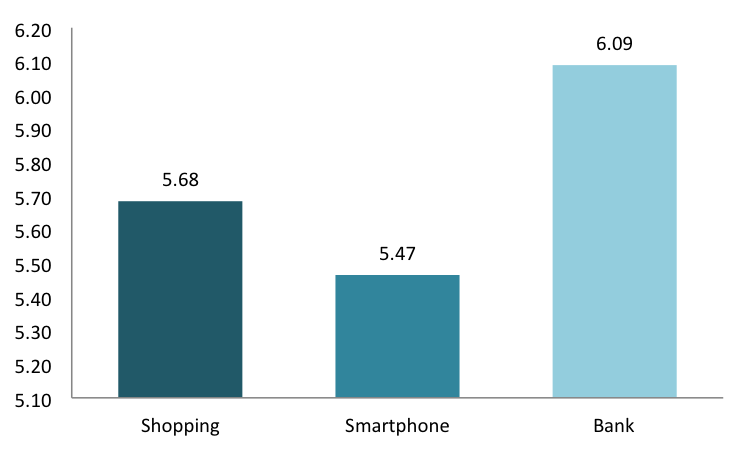
\includegraphics[width=0.45\textwidth]{pics/analysis/avgpatternlength-gender-male.png}
    		\label{fig:avgpatternlengthmale}
    	}
    	\subfigure[Female]{
    		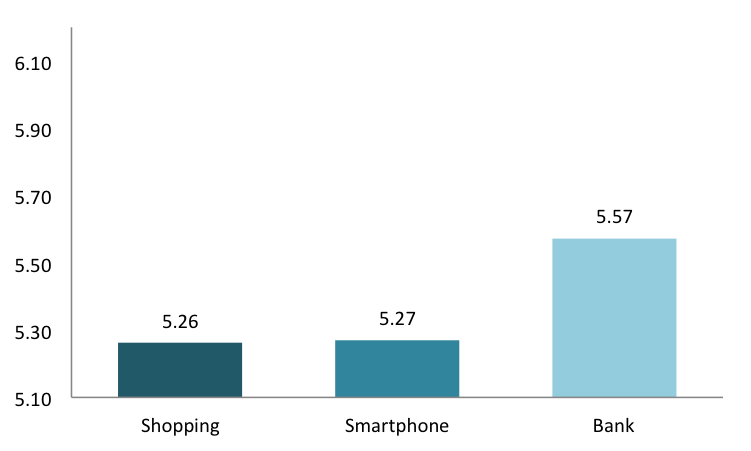
\includegraphics[width=0.45\textwidth]{pics/analysis/avgpatternlength-gender-female.png}
    		\label{fig:avgpatternlengthfemale}
    	}
    	\caption{Average pattern length for gender}
    	\label{fig:avgpatternlengthgender}
    \end{figure}

    \begin{figure}[H]
    	\centering
    	\subfigure[Male]{
    		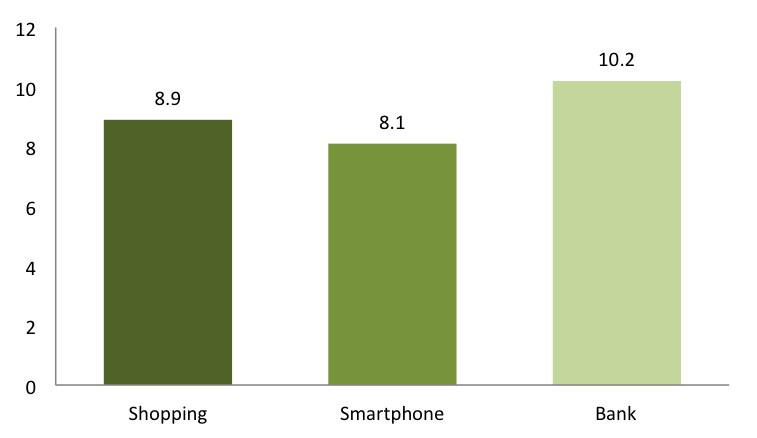
\includegraphics[width=0.45\textwidth]{pics/analysis/creationtime-gender-male.png}
    		\label{fig:avgcreationtimemale}
    	}
    	\subfigure[Female]{
    		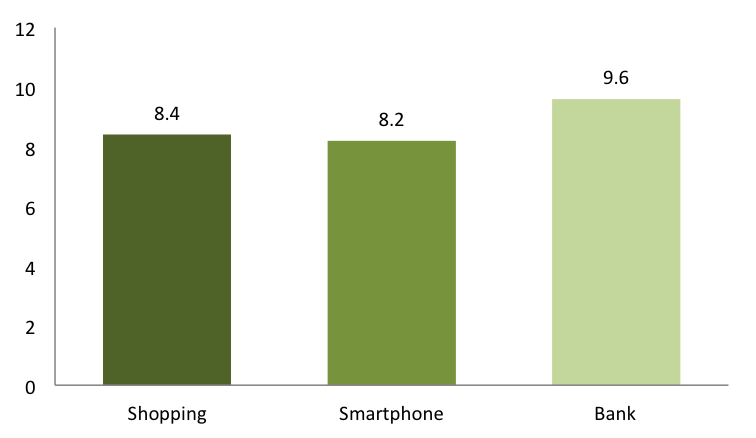
\includegraphics[width=0.45\textwidth]{pics/analysis/creationtime-gender-female.png}
    		\label{fig:avgcreationtimefemale}
    	}
    	\caption{Average pattern creation time for gender}
    	\label{fig:avgcreationtimegender}
    \end{figure}

    \begin{figure}[H]
    	\centering
    	\subfigure[Male]{
    		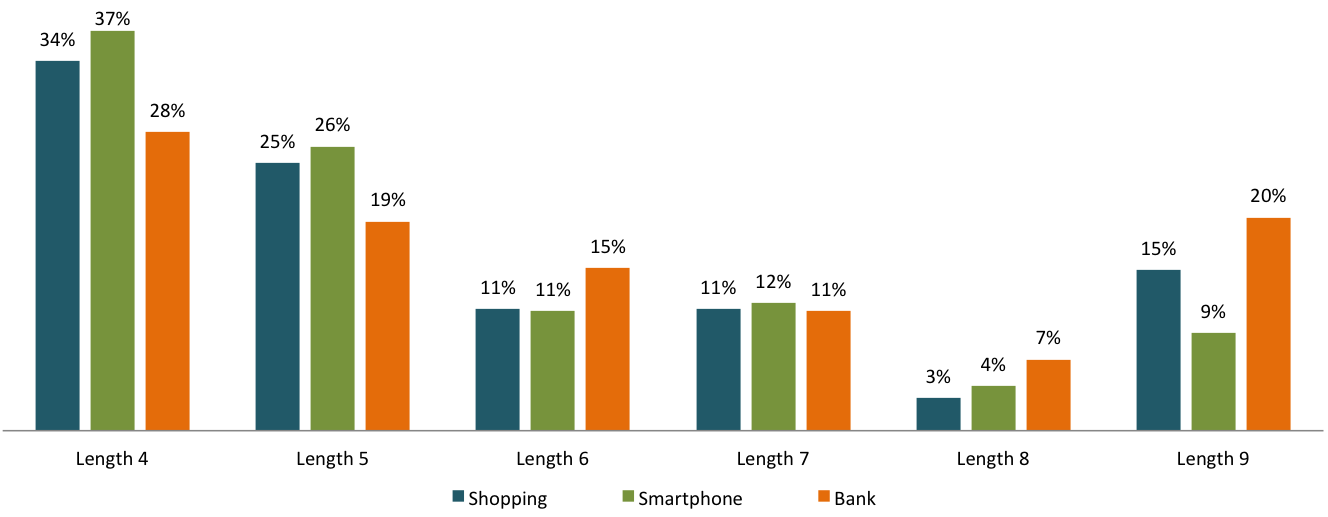
\includegraphics[width=1.0\textwidth]{pics/analysis/patterndist-gender-male.png}
    		\label{fig:avgpatternlengthdistmale}
    	}
    	\subfigure[Female]{
    		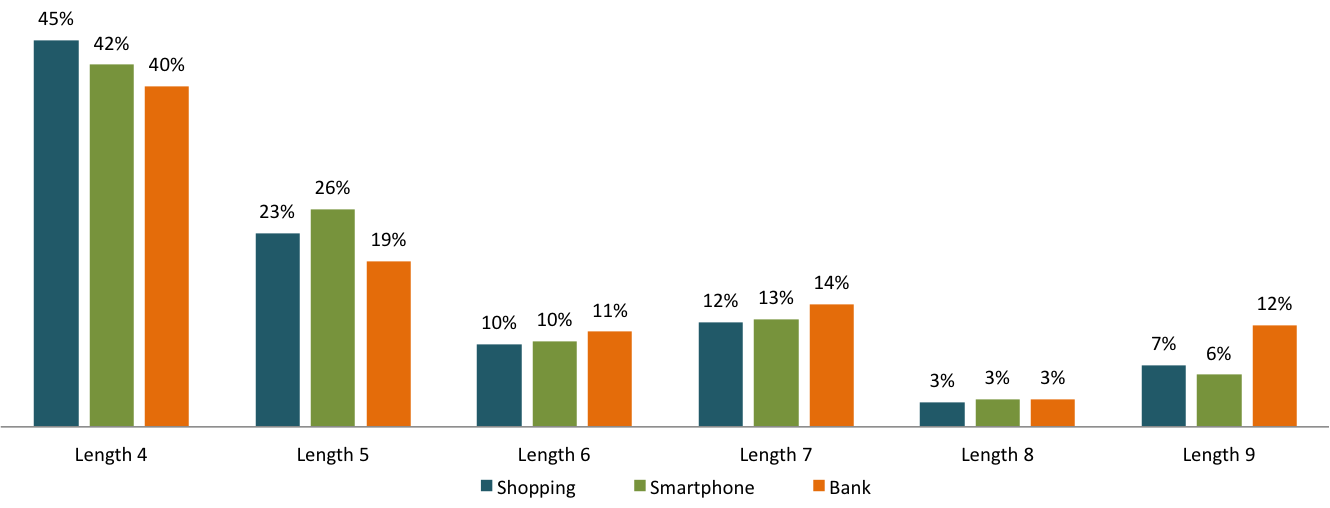
\includegraphics[width=1.0\textwidth]{pics/analysis/patterndist-gender-female.png}
    		\label{fig:avgpatternlengthdistfemale}
    	}
    	\caption{Average pattern length distribution for gender}
    	\label{fig:avgpatterndistgender}
    \end{figure}

	\subsection{Age}

		%Figure: pattern strength based on age
		\begin{figure}[H]
	    \centering
	    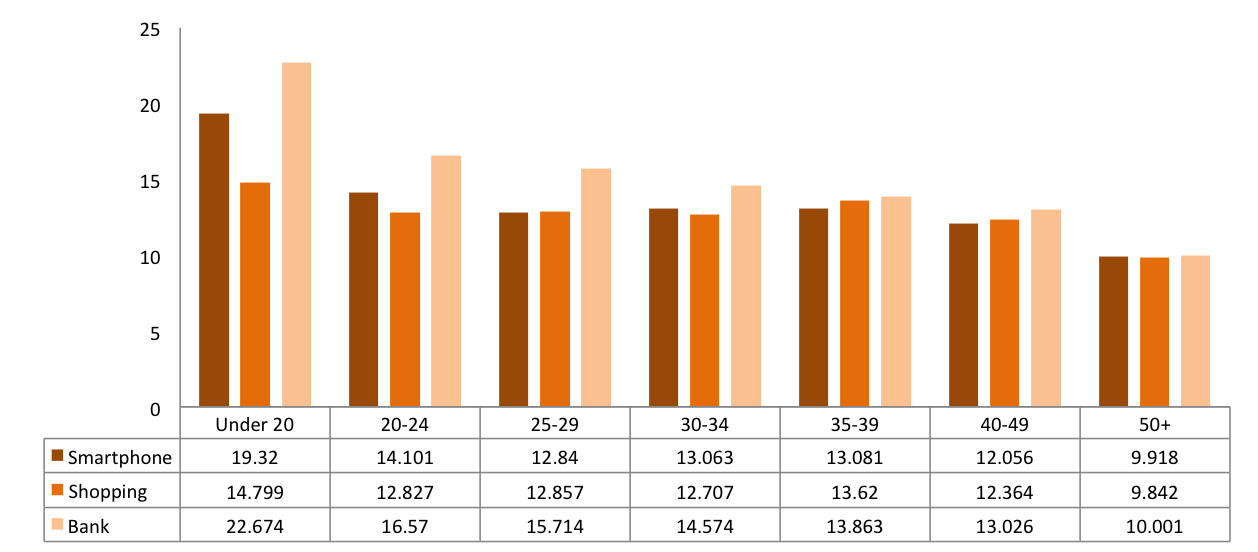
\includegraphics[width=\textwidth]{pics/analysis/strengthagedist.png}
	    \caption{Pattern strength and age distribution}
	    \label{fig:strengthagedist}
  	\end{figure}

  	\begin{figure}[H]
	    \centering
	    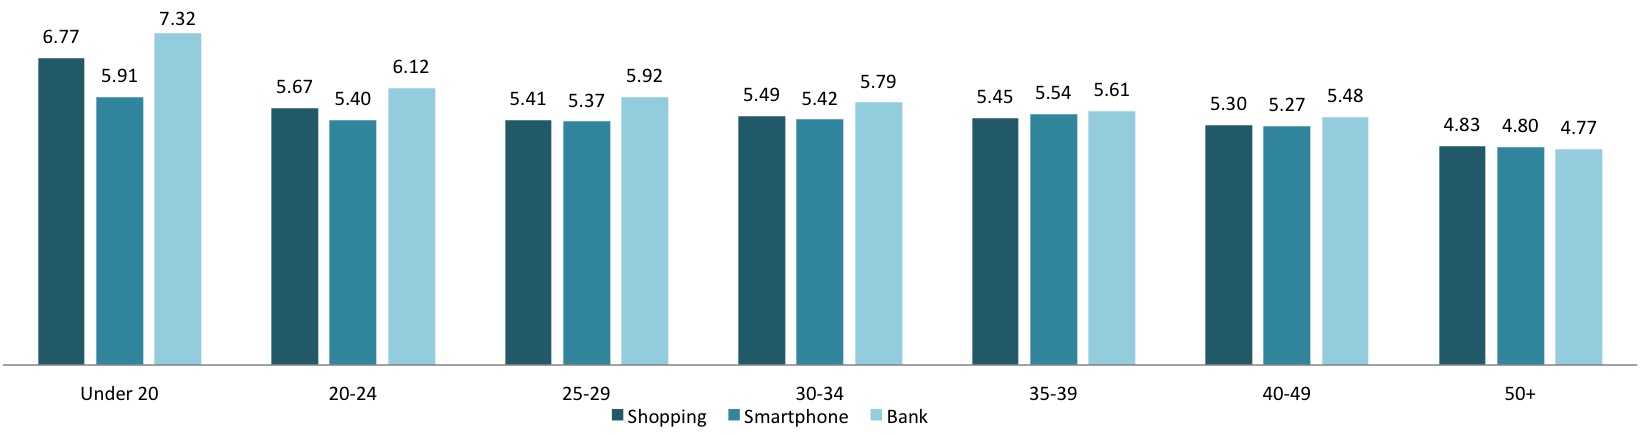
\includegraphics[width=\textwidth]{pics/analysis/avgpatternlength-age.png}
	    \caption{Pattern length by age}
	    \label{fig:patternlengthage}
  	\end{figure}

  	\begin{figure}[H]
	    \centering
	    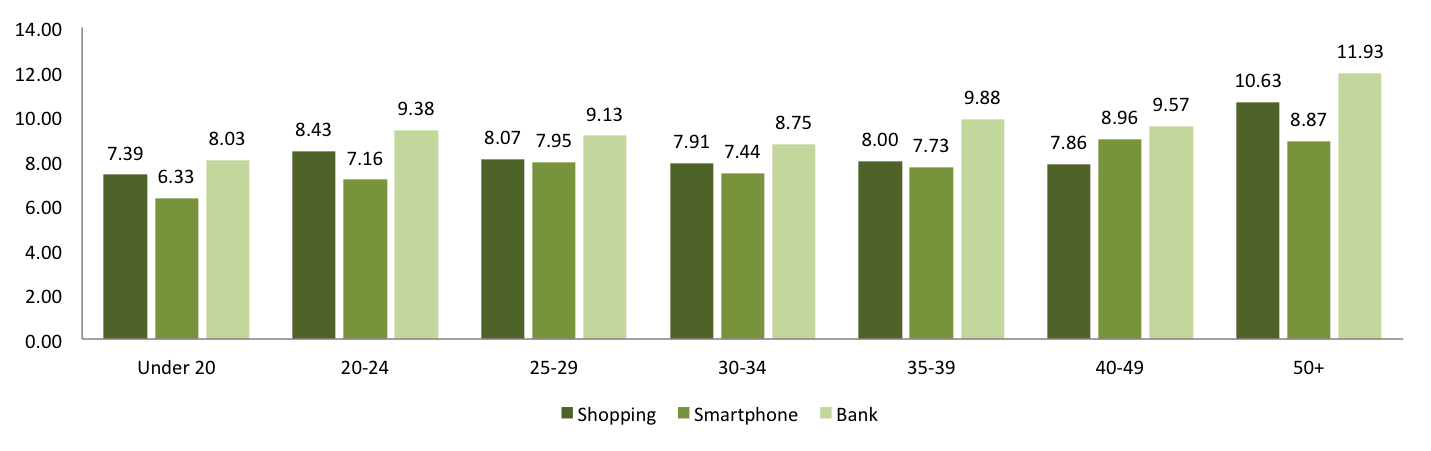
\includegraphics[width=\textwidth]{pics/analysis/creationtime-age.png}
	    \caption{Pattern creation time by age}
	    \label{fig:patterncreationtimeage}
  	\end{figure}

	\subsection{Handedness}
		% Kan her dra inn noe om hvilken hånd og finger som er brukt. 

		\begin{table}[H]
      \centering
      \begin{tabular}{l || l | l || l | l || l | l }
        \hline
         & \multicolumn{2}{c||}{\bf Shopping} & \multicolumn{2}{c||}{\bf Smartphone} &\multicolumn{2}{c}{\bf Bank} \\ \hline
        {\bf Parameters}   & {\bf Right} & {\bf Left} & {\bf Right} & {\bf Left} & {\bf Right} & {\bf Left}\\ \hline
        \#Patterns         & 690 		& 97 			& 690 		& 97 			& 690    & 97     \\
        Avg. Size          & 5.560 	& 5.423 	& 5.423 	& 5.280 	& 5.932  & 5.897  \\
        Avg. Length        & 5.036 	& 5.134 	& 4.966 	& 4.781 	& 5.703  & 5.566  \\
        \#Intersections    & 126 		& 42 			& 124  		& 18 			& 306    & 42     \\
        Avg. Intersections & 0.183 	& 0.433 	& 0.180 	& 0.186 	& 0.443  & 0.433  \\
        \#Overlaps         & 14 		& 0 			& 12 			& 0 			& 18     & 1      \\
        Avg. Overlaps      & 0.020 	& 0.0 		& 0.017 	& 0.0 		& 0.026  & 0.010  \\ \hline
        Avg. Strength      & 13.455 & 13.360 	& 12.966 	& 12.339 	& 15.601 & 15.339 \\ 
        Min strength       & 6.339 	& 6.339 	& 6.339 	& 6.339 	& 6.339  & 6.339  \\
        Max strength       & 39.827	& 44.441 	& 43.187 	& 37.280 	& 44.441 & 44.441 \\ \hline
      \end{tabular}
      \caption{Password strength and handedness}
      \label{tab:handednessstrength} 
    \end{table}

    \begin{figure}[H]
    	\centering
    	\subfigure[Male]{
    		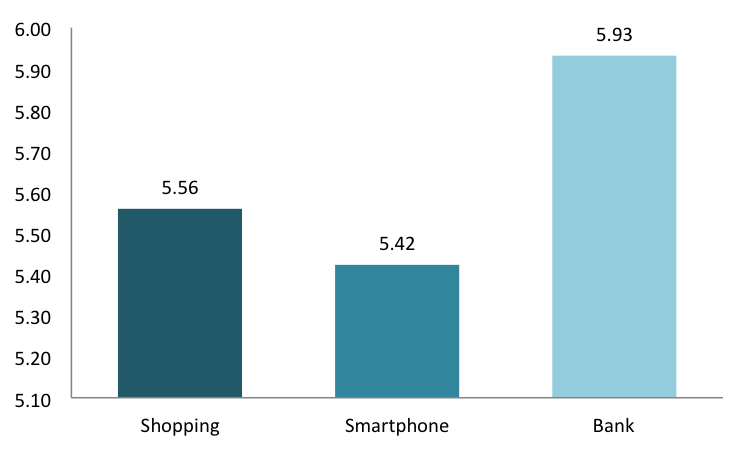
\includegraphics[width=0.45\textwidth]{pics/analysis/avgpatternlength-handedness-right.png}
    		\label{fig:avgpatternlengthright}
    	}
    	\subfigure[Female]{
    		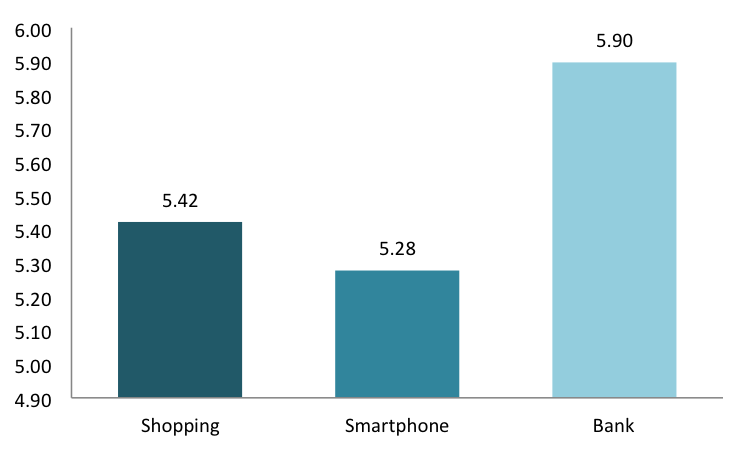
\includegraphics[width=0.45\textwidth]{pics/analysis/avgpatternlength-handedness-left.png}
    		\label{fig:avgpatternlengthleft}
    	}
    	\caption{Average pattern length for handednedd}
    	\label{fig:avgpatternlengthhandedness}
    \end{figure}

    \begin{figure}[H]
    	\centering
    	\subfigure[Male]{
    		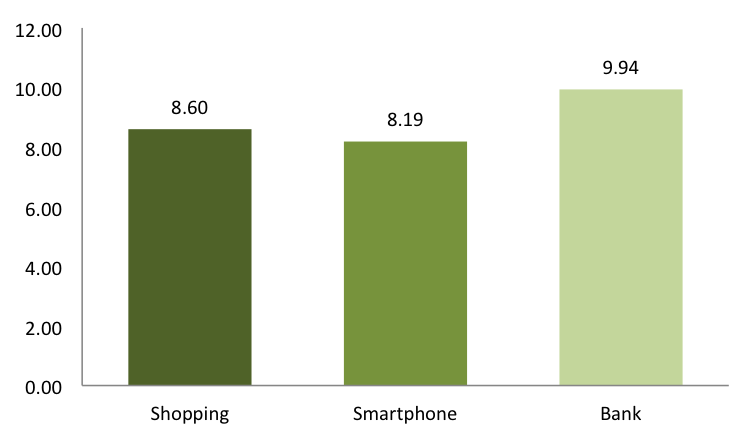
\includegraphics[width=0.45\textwidth]{pics/analysis/creationtime-handedness-right.png}
    		\label{fig:avgcreationtimeright}
    	}
    	\subfigure[Female]{
    		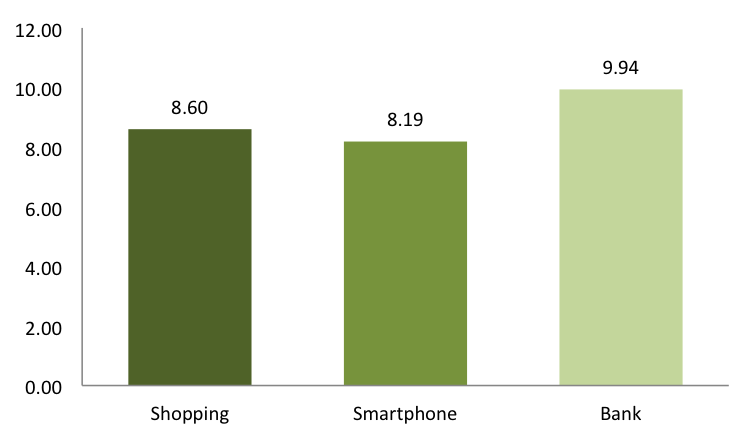
\includegraphics[width=0.45\textwidth]{pics/analysis/creationtime-handedness-right.png}
    		\label{fig:avgcreationtimeleft}
    	}
    	\caption{Average pattern creation time for handedness}
    	\label{fig:avgcreationtimehandedness}
    \end{figure}

    \begin{figure}[H]
    	\centering
    	\subfigure[Male]{
    		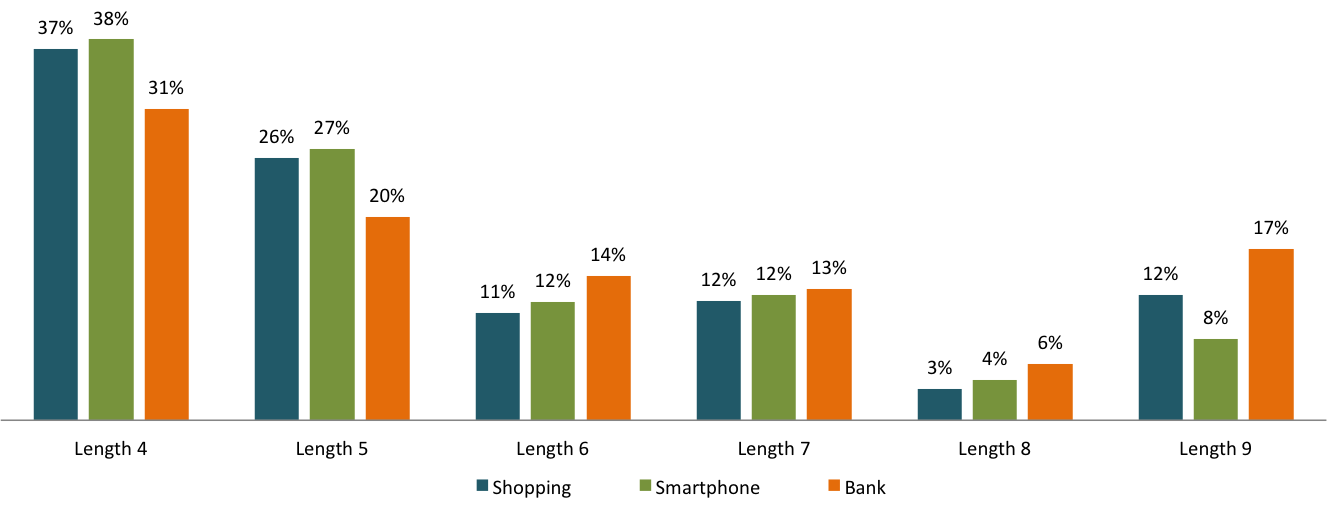
\includegraphics[width=1.0\textwidth]{pics/analysis/patterndist-handedness-right.png}
    		\label{fig:avgpatternlengthdistright}
    	}
    	\subfigure[Female]{
    		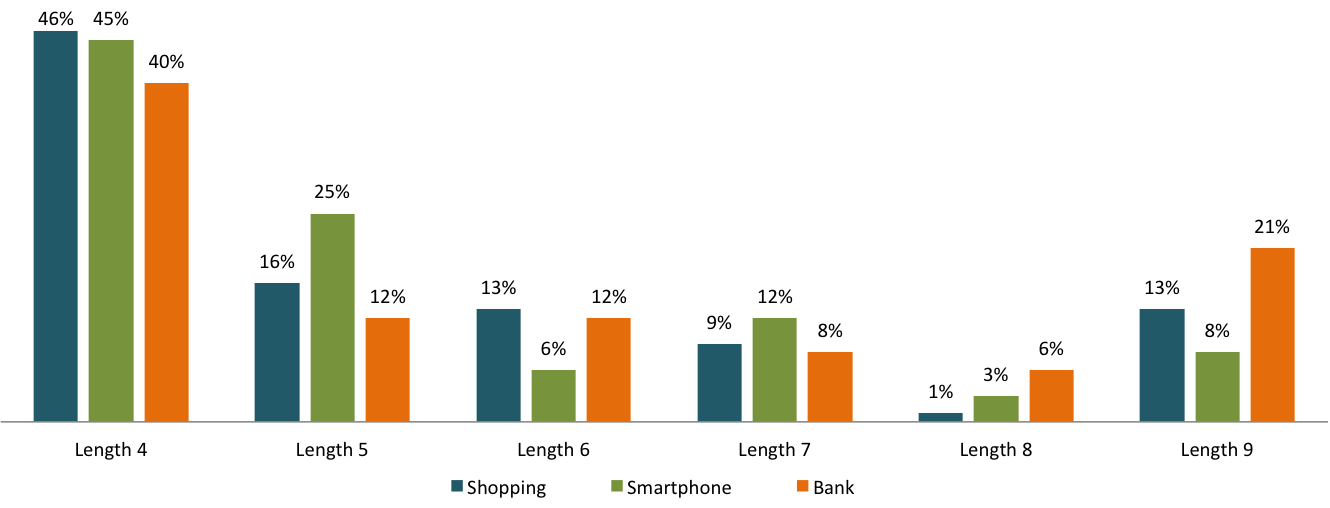
\includegraphics[width=1.0\textwidth]{pics/analysis/patterndist-handedness-left.png}
    		\label{fig:avgpatternlengthdistleft}
    	}
    	\caption{Average pattern length distribution for handedness}
    	\label{fig:avgpatterndisthandedness}
    \end{figure}

		%Table: typing habits, handedness
    \begin{table}[H]
      \parbox{.5\linewidth}{
        \centering
        \begin{tabular}{ l | l | l }
          \hline
          {\bf Hand used} & {\bf Finger used} & {\bf \#} \\ \hline
          \multirow{3}{*}{Right hand} & Thumb & 366 \\
          & Forefinger & 41 \\
          & Other & 8 \\ \hline
          \multirow{3}{*}{Left hand} & Thumb & 33 \\
          & Forefinger & 217 \\
          & Other & 23 \\ \hline
        \end{tabular}
        \caption{{\bf Right-handed} typing habits}
        \label{tab:righthandfinger}
      }
      \hfill
      \parbox{.5\linewidth}{
        \centering
        \begin{tabular}{ l | l | l }
          \hline
          {\bf Hand used} & {\bf Finger used} & {\bf \#} \\ \hline
          \multirow{3}{*}{Right hand} & Thumb & 22 \\ 
          & Forefinger & 26 \\
          & Other & 6 \\ \hline
          \multirow{3}{*}{Left hand} & Thumb & 26 \\ 
          & Forefinger & 10 \\
          & Other & 4 \\ \hline
        \end{tabular}
        \caption{{\bf Left-handed} typing habits}
        \label{tab:lefthandfinger}
      }
    \end{table}

	\subsection{Experience with IT/Security}
		
		\begin{table}[H]
      \centering
      \begin{tabular}{l || l | l || l | l || l | l }
        \hline
         & \multicolumn{2}{c||}{\bf Shopping} & \multicolumn{2}{c||}{\bf Smartphone} &\multicolumn{2}{c}{\bf Bank} \\ \hline
        {\bf Parameters}   & {\bf Yes} & {\bf No} & {\bf Yes} & {\bf No} & {\bf Yes} & {\bf No}\\ \hline
        \#Patterns         & 470    & 332    & 470    & 332    & 470    & 332    \\
        Avg. Size          & 5.636  & 5.386  & 5.479  & 5.274  & 6.113  & 5.605  \\
        Avg. Length        & 5.182  & 4.818  & 5.045  & 4.753  & 5.919  & 5.281  \\
        \#Intersections    & 123    & 41     & 108    & 34     & 231    & 121    \\
        Avg. Intersections & 0.262  & 0.123  & 0.230  & 0.102  & 0.491  & 0.364  \\
        \#Overlaps         & 10     & 4      & 9      & 3      & 13     & 6      \\
        Avg. Overlaps      & 0.021  & 0.012  & 0.019  & 0.009  & 0.028  & 0.018  \\ \hline
        Avg. Strength      & 13.911 & 12.635 & 13.271 & 12.202 & 16.417 & 14.089 \\ 
        Min strength       & 6.339  & 6.339  & 6.339  & 6.339  & 6.339  & 6.339  \\
        Max strength       & 44.441 & 39.827 & 43.187 & 38.870 & 44.441 & 44.441 \\ \hline
      \end{tabular}
      \caption{Password strength and Experience with IT/Security}
      \label{tab:experiencestrength} 
    \end{table}

    \begin{figure}[H]
    	\centering
    	\subfigure[Experience with IT and security]{
    		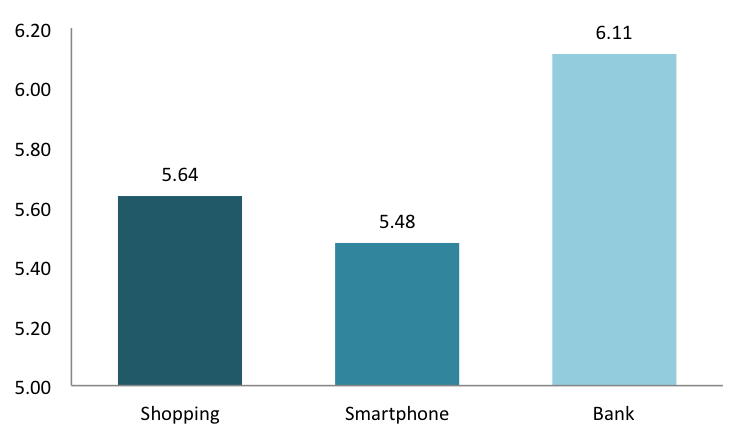
\includegraphics[width=0.45\textwidth]{pics/analysis/avgpatternlength-experience-yes.png}
    		\label{fig:avgpatternlengthyes}
    	}
    	\subfigure[No experience with IT and security]{
    		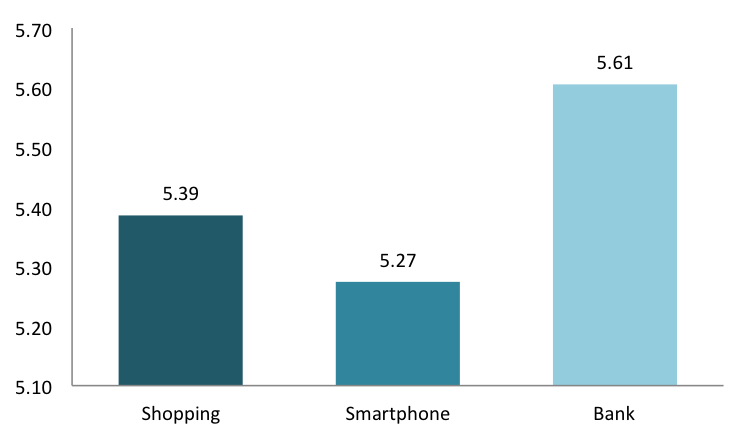
\includegraphics[width=0.45\textwidth]{pics/analysis/avgpatternlength-experience-no.png}
    		\label{fig:avgpatternlengthfeno}
    	}
    	\caption{Average pattern length for experience}
    	\label{fig:avgpatternlengthexperience}
    \end{figure}

    \begin{figure}[H]
    	\centering
    	\subfigure[Male]{
    		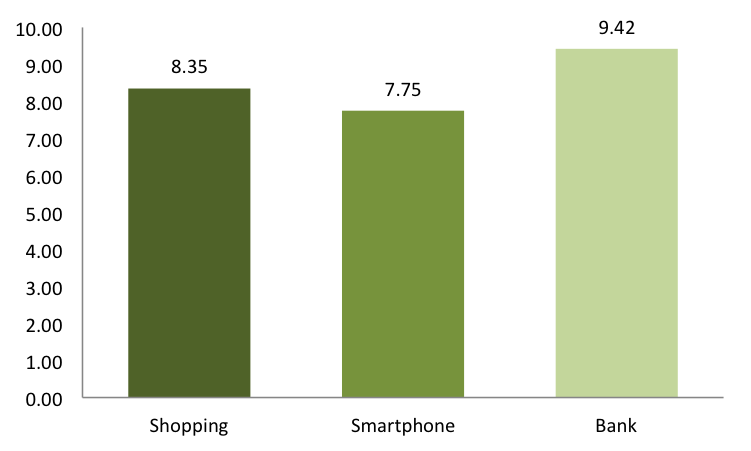
\includegraphics[width=0.45\textwidth]{pics/analysis/creationtime-experience-yes.png}
    		\label{fig:avgcreationtimeyes}
    	}
    	\subfigure[Female]{
    		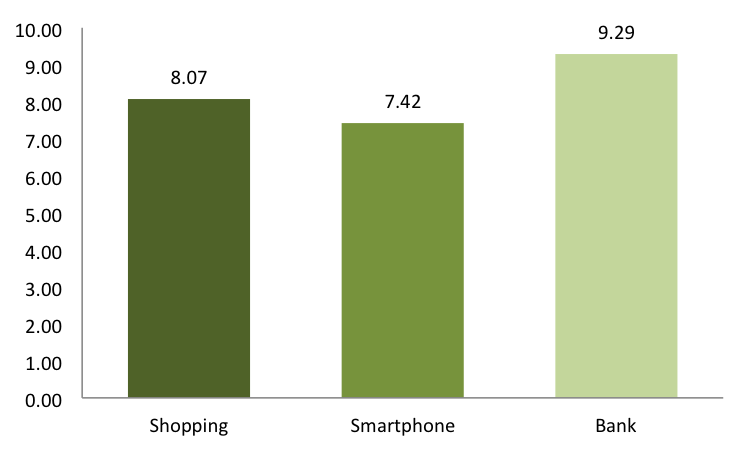
\includegraphics[width=0.45\textwidth]{pics/analysis/creationtime-experience-no.png}
    		\label{fig:avgcreationtimeno}
    	}
    	\caption{Average pattern creation time for Experience}
    	\label{fig:avgcreationtimeexperience}
    \end{figure}

    \begin{figure}[H]
    	\centering
    	\subfigure[Experience with IT and security]{
    		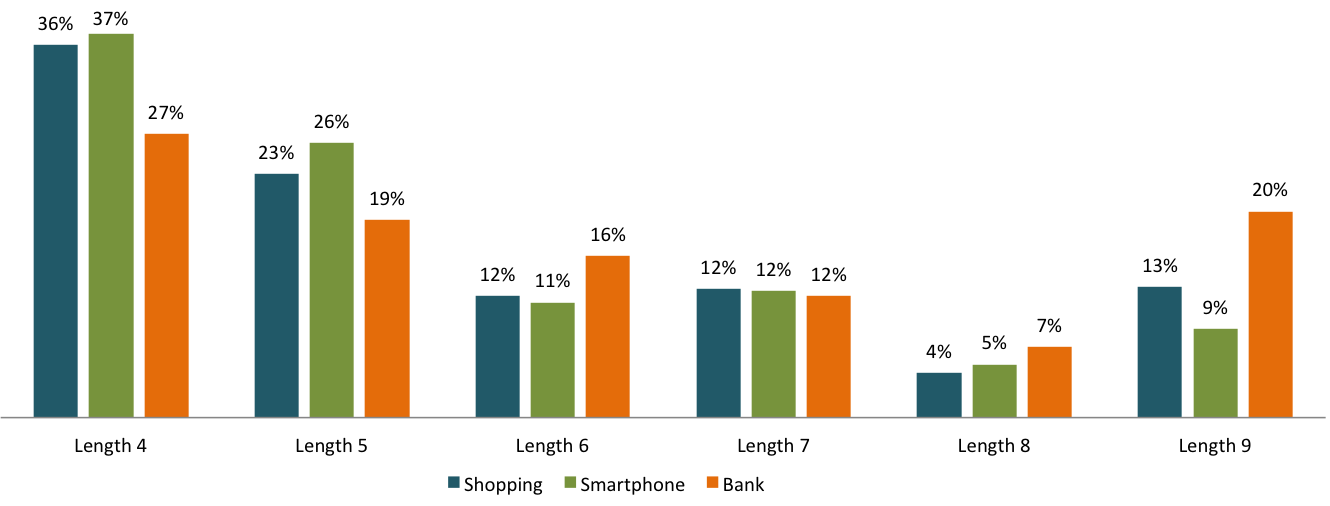
\includegraphics[width=1.0\textwidth]{pics/analysis/patterndist-experience-yes.png}
    		\label{fig:avgpatternlengthdistyes}
    	}
    	\subfigure[No experience with IT and security]{
    		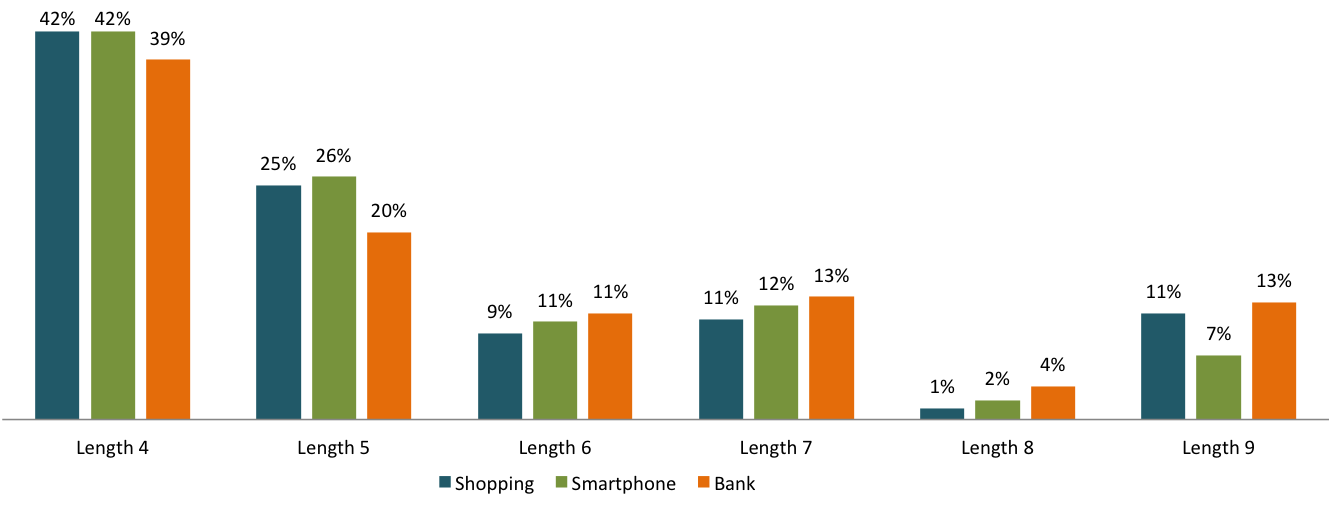
\includegraphics[width=1.0\textwidth]{pics/analysis/patterndist-experience-no.png}
    		\label{fig:avgpatternlengthdistno}
    	}
    	\caption{Average pattern length distribution for experience}
    	\label{fig:avgpatterndistexperience}
    \end{figure}


